\chapter{提案モデルによる日本近辺の風速予測\label{chap:experiments}}
本論文では,提案モデルの性能検証のために日本近辺の風速予測を実施した.また,性能の比較のためにCNNによるエンコーダ・デコーダとLSTMを用いたモデルを実装し,それぞれのモデルの性能を比較した.

\section{実験の概要 \label{section:exp-overview}}
ここに何をメトリクスとして取ったのかとかを書く

\section{利用したデータ及び学習条件 \label{section:exp-data-and-condition}}
\subsection{利用したデータ \label{subsection:exp-data}}
気象庁が提供している日本近辺の風速と気圧データを京都大学の生存圏データベース\cite{Seizonken2004}から入手した.このデータセットは図\ref{fig:exp-data-overview}に示す通り,日本近辺の北緯$22.4\tcdegree$から$47.6\tcdegree$まで,東経$120\tcdegree$から$150\tcdegree$までの領域をそれぞれ$0.05\tcdegree \times 0.0625\tcdegree$の細かさで等緯度等経度に区切り,各格子点上における風速と気圧を記録したものである\cite{JMBSC2022}.すなわち,ある一時刻のデータは緯度経度について$505 \times 480$の行列となっており,ある一点には風速の南北方向成分$(\mathrm{m/s})$, 風速の東西方向成分$(\mathrm{m/s})$, 気圧$(\mathrm{hPa})$の3つの値が記録されている.
\begin{figure}[btp]
  \centering
  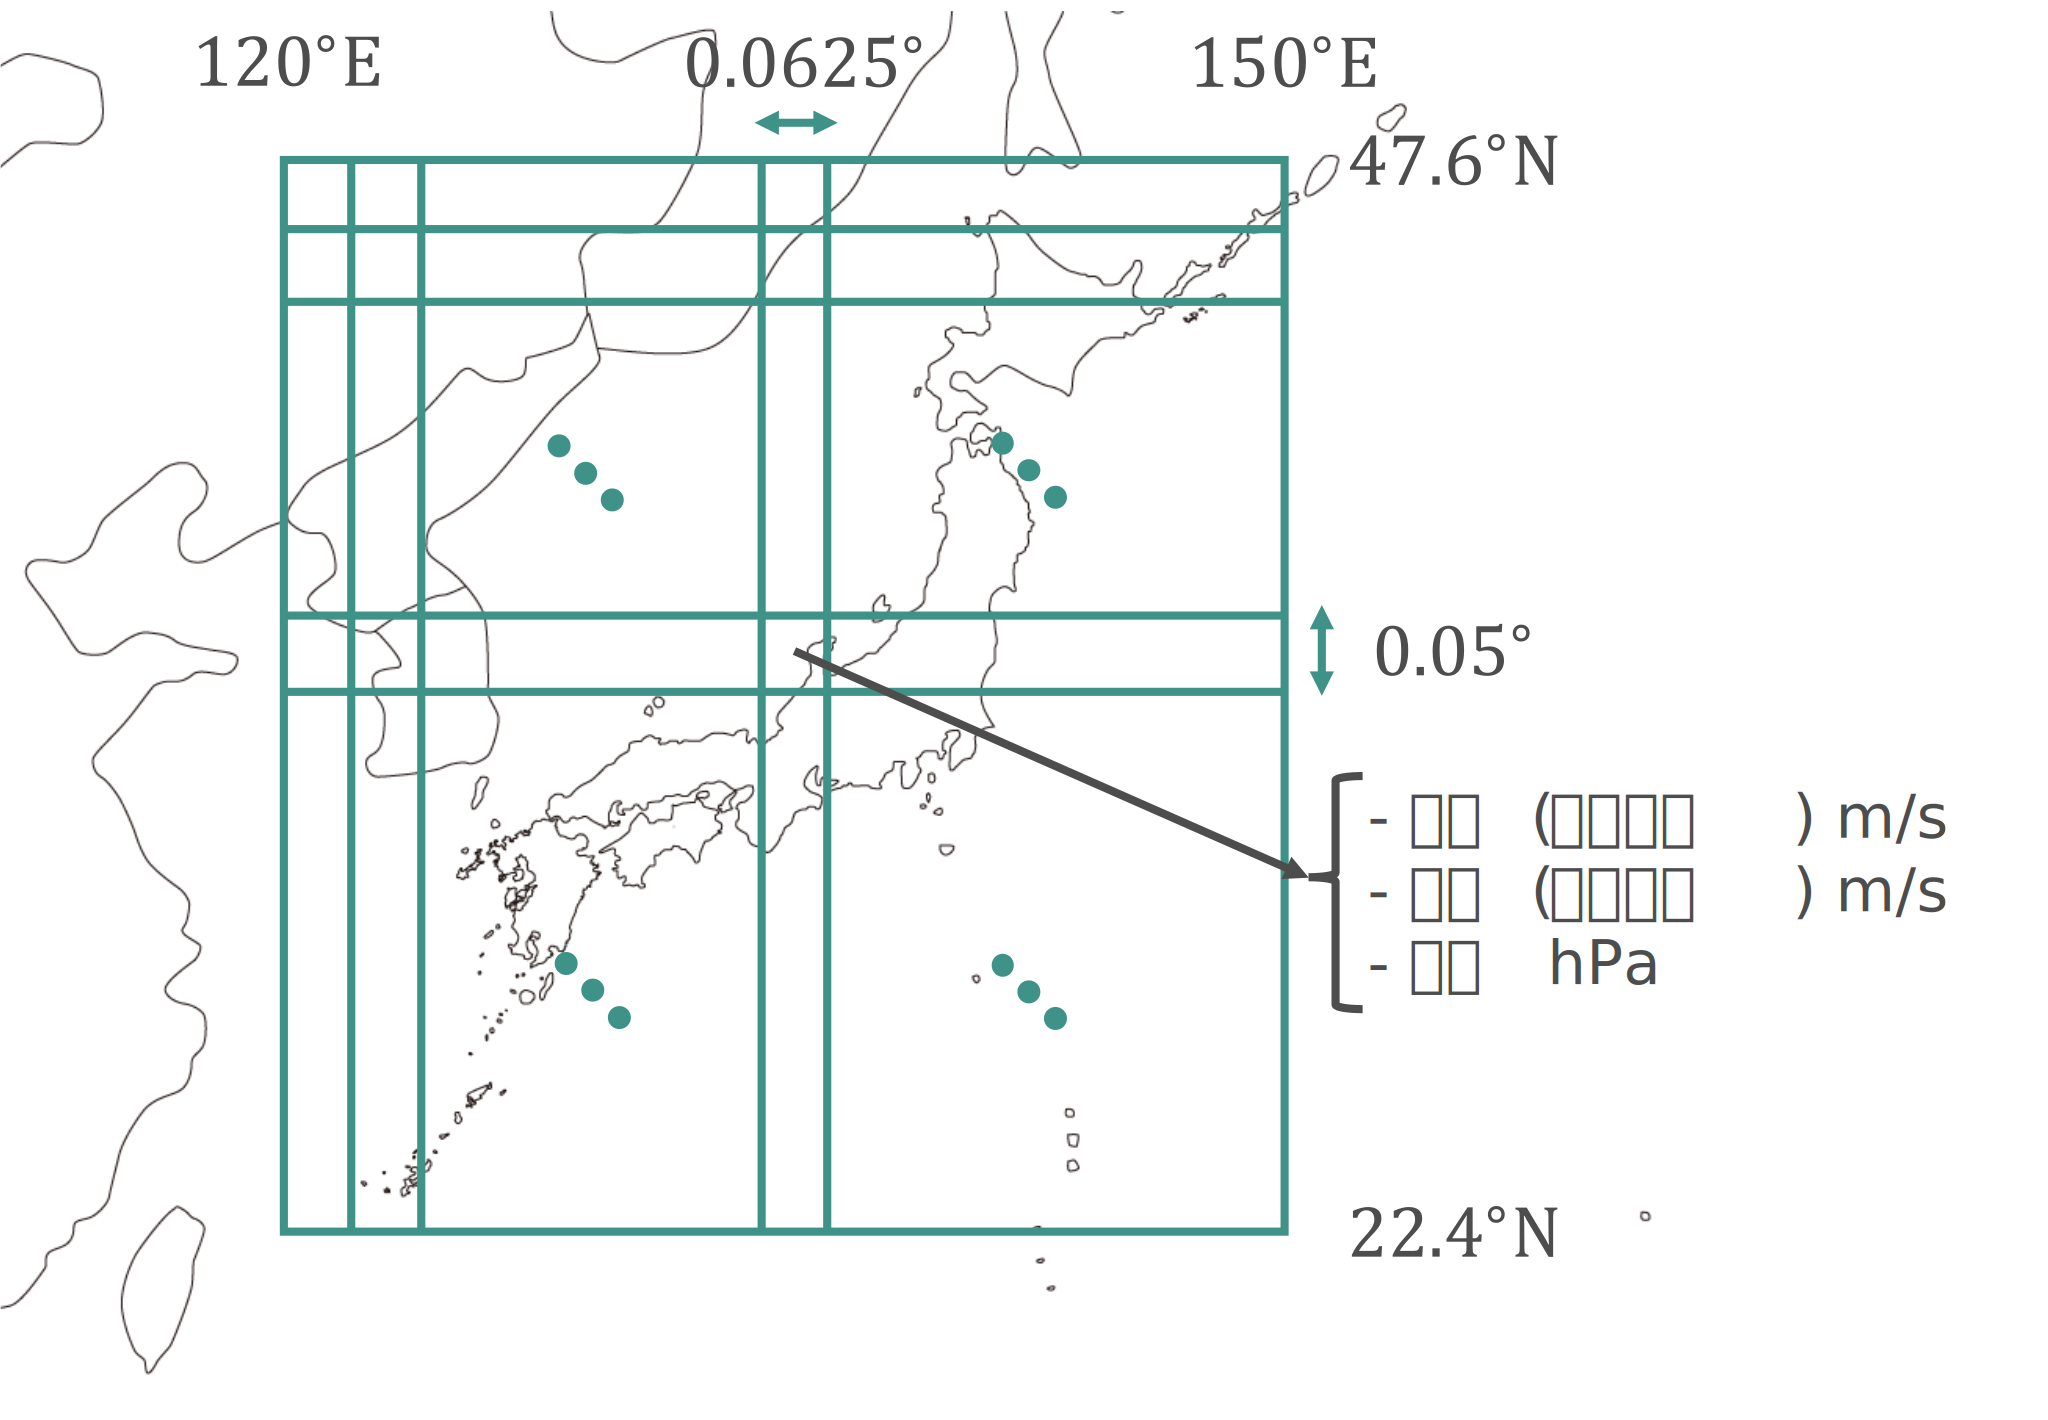
\includegraphics[width=0.6\linewidth]{./experiments/figs/data_overview.svg.eps}
  \caption{気象庁が提供している日本近辺の風速と気圧データの領域}
  \label{fig:exp-data-overview}
\end{figure}

今回の時系列データは3時間間隔であり,(前日の)21:00, 0:00, 3:00の3時刻分のデータを入力として6:00の時刻の風速を予測するというタスクを行った.すなわち,式(\ref{eq:time-series-input})において$n=5$,式(\ref{eq:time-series-t})において$\Delta T$は$3[\mathrm{h}]$相当である.この4時刻分の時系列データを2011年1月1日から2020年12月31日までの3650日分用意し(統計を取る際の簡便化のために閏日は除いてある),全体のデータセットとした.

データセットの詳細な統計量を表\ref{todo:table:exp-data-statistics}に示す.

\subsection{データの前処理 \label{subsection:exp-data-preprocessing}}
\ref{subsection:exp-data}項で述べたデータセットをそのまま入出力として用いるのではなく,いくつかの前処理を実施した.その処理の詳細を以下に示す.

まず$505 \times 480$の行列を更に$10 \time 10$の格子によって区切り,この格子内で風速と気圧を平均化することで$50 \times 48$のサイズまで落とした(図\ref{}).これは,提案モデルの格子の大きさを適切に設定することで,3時間で変化する風速の空間的な変化を捉えることができると考えたためである.

続いて,風速と気圧の値をそれぞれ標準化した.これは,風速と気圧の値のスケールが異なるため,それぞれの値を標準化することで,モデルの学習を安定化させるためである.

\subsection{学習条件 \label{subsection:exp-condition}}

続いて,モデルの詳細なハイパーパラメータの設定について述べる.

提案モデルの学習にはAdam\cite{Kingma2014AdamAM}を用いた.学習率は$10^{-3}$とし,ミニバッチサイズは$16$とした.全体のデータセットを2920日分と730日分に分けそれぞれを学習用データと検証用データとした.学習は$500$エポック行い,かかった時間は約8時間であった.実行環境にはGoogle Colaboratory\cite{GoogleColaboratory}を用い,GPUはTesla T4を用いた.また提案モデルの構築にはPyTorch\cite{NEURIPS2019-9015}を用い,自動微分による学習を行った.

\section{実験結果 \label{section:exp-results}}

\section{物理的な構造を含まない深層学習モデルによる実験結果 \label{section:exp-results-without-physicial-structure}}

\section{考察 \label{section:exp-discussion}}
% 平均化についてもふれて,どうやって